% -----------------------------------------------
% Template for SMAC SMC 2013
% adapted and corrected from the template for SMC 2012, which was adapted from that of SMC 2011
% further updated for TENOR 2015, 2016 and 2017
% -----------------------------------------------

\documentclass{article}
\usepackage{tenor2017}
\usepackage{ifpdf}
\usepackage[english]{babel}
\usepackage{balance}
\usepackage{courier}

\newcommand{\code}[1]{\texttt{#1}}
%%%%%%%%%%%%%%%%%%%%%%%% Some useful packages %%%%%%%%%%%%%%%%%%%%%%%%%%%%%%%
%%%%%%%%%%%%%%%%%%%%%%%% See related documentation %%%%%%%%%%%%%%%%%%%%%%%%%%
%\usepackage{amsmath} % popular packages from Am. Math. Soc. Please use the 
%\usepackage{amssymb} % related math environments (split, subequation, cases,
%\usepackage{amsfonts}% multline, etc.)
%\usepackage{bm}      % Bold Math package, defines the command \bf{}
%\usepackage{paralist}% extended list environments
%%subfig.sty is the modern replacement for subfigure.sty. However, subfig.sty 
%%requires and automatically loads caption.sty which overrides class handling 
%%of captions. To prevent this problem, preload caption.sty with caption=false 
%\usepackage[caption=false]{caption}
%\usepackage[font=footnotesize]{subfig}


%%%%%%%%%%%%%%%%%%%%%%%% Some useful packages %%%%%%%%%%%%%%%%%%%%%%%%%%%%%%%
%%%%%%%%%%%%%%%%%%%%%%%% See related documentation %%%%%%%%%%%%%%%%%%%%%%%%%%
%\usepackage{amsmath} % popular packages from Am. Math. Soc. Please use the 
%\usepackage{amssymb} % related math environments (split, subequation, cases,
%\usepackage{amsfonts}% multline, etc.)
%\usepackage{bm}      % Bold Math package, defines the command \bf{}
%\usepackage{paralist}% extended list environments
%%subfig.sty is the modern replacement for subfigure.sty. However, subfig.sty 
%%requires and automatically loads caption.sty which overrides class handling 
%%of captions. To prevent this problem, preload caption.sty with caption=false 
%\usepackage[caption=false]{caption}
%\usepackage[font=footnotesize]{subfig}


%user defined variables
\def\papertitle{A Hierarchic Diff Algorithm for Collaborative Music Document Editing}
\def\firstauthor{Christopher Antila}
\def\secondauthor{Jeffrey Trevi\~{n}o}
\def\thirdauthor{Gabriel Weaver}

% adds the automatic
% Saves a lot of ouptut space in PDF... after conversion with the distiller
% Delete if you cannot get PS fonts working on your system.

% pdf-tex settings: detect automatically if run by latex or pdflatex
\newif\ifpdf
\ifx\pdfoutput\relax
\else
   \ifcase\pdfoutput
      \pdffalse
   \else
      \pdftrue
\fi

\ifpdf % compiling with pdflatex
  \usepackage[pdftex,
    pdftitle={\papertitle},
    pdfauthor={\firstauthor, \secondauthor, \thirdauthor},
    bookmarksnumbered, % use section numbers with bookmarks
    pdfstartview=XYZ % start with zoom=100% instead of full screen; 
                     % especially useful if working with a big screen :-)
   ]{hyperref}
  %\pdfcompresslevel=9

  \usepackage[pdftex]{graphicx}
  % declare the path(s) where your graphic files are and their extensions so 
  %you won't have to specify these with every instance of \includegraphics
  \graphicspath{{./figures/}}
  \DeclareGraphicsExtensions{.pdf,.jpeg,.png}

  \usepackage[figure,table]{hypcap}

\else % compiling with latex
  \usepackage[dvips,
    bookmarksnumbered, % use section numbers with bookmarks
    pdfstartview=XYZ % start with zoom=100% instead of full screen
  ]{hyperref}  % hyperrefs are active in the pdf file after conversion

  \usepackage[dvips]{epsfig,graphicx}
  % declare the path(s) where your graphic files are and their extensions so 
  %you won't have to specify these with every instance of \includegraphics
  \graphicspath{{./figures/}}
  \DeclareGraphicsExtensions{.eps}

  \usepackage[figure,table]{hypcap}
\fi

%setup the hyperref package - make the links black without a surrounding frame
\hypersetup{
    colorlinks,%
    citecolor=black,%
    filecolor=black,%
    linkcolor=black,%
    urlcolor=black
}


% Title.
% ------
\title{\papertitle}

% Authors
% Please note that submissions are NOT anonymous, therefore 
% authors' names have to be VISIBLE in your manuscript. 
%
% Single address
% To use with only one author or several with the same address
% ---------------
%\oneauthor
%   {\firstauthor} {Affiliation1 \\ %
%     {\tt \href{mailto:author1@adomain.org}{author1@adomain.org}}}

%Two addresses
%--------------
% \twoauthors
%   {\firstauthor} {Affiliation1 \\ %
%     {\tt \href{mailto:author1@adomain.org}{author1@adomain.org}}}
%   {\secondauthor} {Affiliation2 \\ %
%     {\tt \href{mailto:author2@adomain.org}{author2@adomain.org}}}

% Three addresses
% --------------
 \threeauthors
   {\firstauthor} {nCoda \\ %
     {\tt \href{mailto:christopher@antila.ca}{christopher@antila.ca}}}
   {\secondauthor} {California State University, Monterey Bay \\ %
     {\tt \href{mailto:jtrevino@csumb.edu}{jtrevino@csumb.edu}}}
   {\thirdauthor} { University of Illinois, Urbana-Champaign \\ %
     {\tt \href{mailto:gweaver@illinois.edu}{gweaver@illinois.edu}}}


% ***************************************** the document starts here ***************
\begin{document}
%
\capstartfalse
\maketitle
\capstarttrue
%
\begin{abstract}
We describe an application of hierarchic diff to the collaborative
editing of tree-based music representations, using Zhang and Shasha's
tree edit distance algorithm as implemented within the XUDiff tool.
The edit distance between two trees is the minimum number of edit
operations necessary to transform one tree into the other.  We
consider common operations on the score tree---deleting, changing, and
appending tree nodes----to derive a minimal edit sequence, known as an
edit script, and we compare the performance of the widely used Longest
Common Subsequence algorithm against our approach.
\end{abstract}
%

\section{Introduction}\label{sec:introduction}
\subsection{The Longest Common Subsequence Algorithm as Default Diff}
Traditional document comparison algorithms, such as in the Unix
\texttt{diff} program, take two sequences of characters as input, and
output an edit script to transform one sequence into the other.  An
\emph{edit script} consists of a sequence of edit operations (usually
insert, delete, and update) to transform the first sequence relative
to some entity---usually characters, words, or lines.  The \emph{edit
  distance} is the minimum cost the edit script gives for each
operation.  The Longest Common Subsequence algorithm and its variants
are the most common for computing an edit script and cost.

The Longest Common Subsequence algorithm works well in situations where
the inputs are sequences of characters and one wants to be
able to compare those sequences relative to characters, words, or
lines, but many modern file formats rely on
hierarchical object models to encode multiple levels of meaning
(e.g. XML, blocks of code).  As such, different algorithms for
hierarchical structures become necessary.  

Consider the following two problems that result from this mismatch
between character- or line-based diff tools and tree-structured input.
First, comparing documents in terms of low-level entities
(e.g. lines) may not result in changes that are meaningful to the
domain, because lines are often an artifact of presentation: for
example, one can generate 'noisy diffs' by just changing whitespace.
Second, the manner in which one defines document similarity may change
depending upon the task at hand.  A poet may get along fine comparing
texts in terms of lines, which reflect part of the structure of the
text.  A musician, however, may want to compare documents in terms of
additional information that is lost from a purely line-based approach.
A similar demand is seen within other communities; scholars may want
to analyze and compare texts relative to other structures, such as
paragraphs or sections.

\subsection{Collaborative Music Information Requires a Hierarchic Diff}
As alluded to above, these problems are of specific importance to
those in music, both in terms of usability as well as how one may want
to define 'meaning' and 'similarity' among musical documents.  First,
the 'noisy diff' problem---in reporting differences that are not
relevant to musicians---creates a usability problem.  Although
programmers have become accustomed to noisy diffs and the work-arounds
they require, the low adoption rate of computer-driven music analytic
tools, and the general lack of comfort among music scholars with these
tools, suggest that a program producing diffs of meaningless changes
would be poorly received by the community.  Second, the meaning of
textually encoded music always requires additional interpretation.
Therefore, a one-dimensional sequence of characters (the data
structure for which traditional diff was designed) will not allow
musicians to compare two interpretations of music.  

Instead, musicians need the ability to compare musical information in
the presence of its logical organization, which must be expressed
hierarchically.  Therefore, musicians need the ability to compare two
versions of a hierarchical structure.  Finally, musicians may want to
compare two versions of a score at different levels of abstraction, as
represented by these hierarchical structures, or restrict comparison
to entities with certain properties: for example, a musician may want
to compare two versions of a score in terms of pitch class alone, or
of higher-level features like phrase structure. Moreover, a musician
may want to filter a score to compare two versions of only a single
instrument's staff within a score, and other musical abstractions that
require an algorithm to filter the score's hierarchical
representation.

\subsection{Precedents in the Music Literature}
<<<<<<< HEAD
Few relevant precedents exist in the literature, for the reason that music document creation systems assume a single user by default -- collaborative music document creation should still be regarded as an experimental pursuit, and precedents fall largely into the category of systems for experimental music composition. Within these experimental systems, version control for distributed workflows seems to have been avoided by system design choices, and the semantic-aware navigation of tree-based information representations seems to have largely been obviated by system design choices. Jord\`{a} and W\''{u}st base their online collaborative composition system on tree-based, XML representations, but they do not mention version control


\section{Applying The Zhang and Shasha Algorithm}
\subsection{The Zhang and Shasha Algorithm}
Our initial approach uses Zhang and Shasha's tree edit distance
algorithm as implemented within the \texttt{XUDiff} tool
\cite{Weaver:2013sl}.  The edit distance between two trees is the
minimum number of edit operations necessary to transform one tree to
another.  The edit operations we consider include deletion, change,
and appending of tree nodes.  As before, a sequence of edit operations
between two trees is called an \emph{edit script}.

Our proposed approach leverages previous work from other domains in both
industry and in academia.  Within industry, there are proprietary,
hierarchy-aware difference engines that compare source code in a variety of 
edit operations, such as the SmartDifferencer by Semantic Designs
\cite{Designs:qm}.  Within academia, the tree diffing problem has been
long studied by theoretical computer science \cite{Bille:2005ec}.
Researchers such as Chawathe et al. and Cobena et
al. have studied alternative algorithms, such as subtree hashing, 
and even the use of IDs to align subtrees before similarity 
computation \cite{Chawathe:1996jb,Cobena:2002gd}.  We employ the Zhang 
and Shasha tree difference algorithm to solve the edit distance between
trees \cite{Zhang:1989ec,Zhang:1989il}.

There are several benefits to the Zhang and Shasha tree edit
difference algorithm.  First, the algorithm produces a tree edit
distance that is a metric if the cost function is also a metric.  A
distance metric is desirable because collaborators can use it to
explore the similarity of an entire corpus of musical scores---rather
than just two scores---because the metric's notion of distance aligns
with our intuition about distance in the physical world.  Second, the
algorithm is relatively simple and as such, lends itself to a
straightforward implementation that can be maintained by an
open-source community.  The intent of the open-source community is to
support an extensible framework for hierarchical comparision of a wide
variety of document types across a number of domains.  In the future,
other algorithms, such as those mentioned above, may be implemented to
understand more about the effect of different tree-edit distance
algorithms on similarity results.

(Idea for Jeffery and Christopher:  Perhaps insert citations from the research space of topology
of musical data.  Also, we could discuss the practical benefits of
this approach (hierarchcial diffing) as well as the benefit to
collaborative composition as this would allow people to understand how
and in what manner their music differs from a whole corpus of pieces
and simultaneously enable research in topological spaces for musical objects.)

One benefit of this approach is that practitioners can choose a
preferred level of abstraction (as defined by level within the tree)
with which to summarize a change and define 'similarity'.  As such, we
hypothesize that XUDiff, when applied to interpretations of music as
hierarchically encoded by the MEI object model, will be able to
address the problems mentioned above: comparing score changes in terms
of their semantic organization, via the algorithm's hierarchical
interpretation of the text, which yields less noisy comparisons.

\begin{figure}[!htb]
\centering
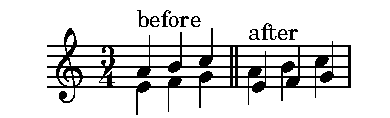
\includegraphics[width=0.7\columnwidth]{layers.pdf}
\caption{An edit that switches the first and second voices in a staff. Stem direction is the only visual difference, but the underlying representation changes substantially.}
\label{fig:voice_swap}
\end{figure}

\subsection{A Comparative Example}
Consider the case of a simple edit: exchanging a staff's two voices.
That is, as shown in Figure~\ref{fig:voice_swap}, the upward-facing
stems of voice one become the downward-facing stems of voice two, and
vice versa.

While Common Western Notation displays only a change of stem
direction, a tree-based, hierarchic representation of this musical
information must alter both the labeling and succession of elements.
In the MEI XML representation of a music document, the voice-switch
example may be encoded in the following way:


\begin{verbatim}
<staff n="1"> 
    <layer n="1">
        <note pname="a"/>
        <note pname="b"/>
        <note pname="c"/>
    </layer>
    <layer n="2">
        <note pname="e"/>
        <note pname="f"/>
        <note pname="g"/>
    </layer>
</staff>
\end{verbatim}

becomes:

\begin{verbatim}

<staff n="1">
    <layer n="1">
        <note pname="e"/>
        <note pname="f"/>
        <note pname="g"/>
    </layer>
    <layer n="2">
        <note pname="a"/>
        <note pname="b"/>
        <note pname="c"/>
    </layer>
</staff>
\end{verbatim}


\subsection{Comparing LCS against Zhang and Shasha Performance}
This example, although basic, motivates the need to to compare representations of music in terms of its 
hierarchical structure, rather than line-by-line. Figure~\ref{fig:lcs-diff} illustrates an edit script that maps one
version of an MEI-encoded score to another in terms of lines.
The line-based approach successfully captures the need to switch the
notes in layer 1 and layer 2, however additional noise is added
because \code{diff} compares the MEI rather than the hierarchical
structure encoded by the MEI.  As a result, the total edit distance is
10.  If practitioners are interested in understanding change relative
to the hierarchical object model of MEI, they will need to sift
through the noisy changes produced by a line-based comparison.  As
mentioned earlier, this may be problematic for widespread adoption
within the music community.

\begin{figure}[ht]
\centering
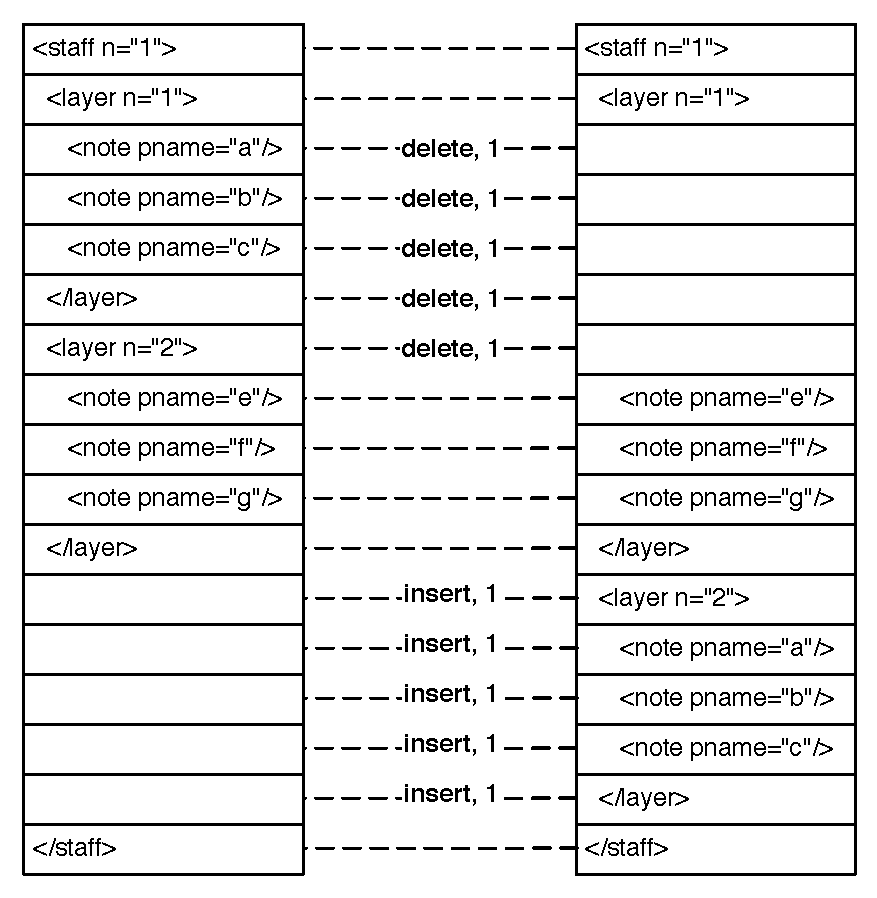
\includegraphics[scale=0.5]{figures/lcs-diff.pdf}
\caption{The figure above illustrates the output of \code{diff}
  applied to MEI.  A total edit distance of 10 results from updating
  the notes in layer 1 and layer 2 (cost of 6), as well as updating
  \code{layer} tags (cost of 4).  Nearly half of the edit distance is
  'noise' from deleting lines with \code{layer} tags, an artifact of
  comparing versions in terms of lines instead of MEI elements.}
\label{fig:lcs-diff}
\end{figure}

\begin{figure}[h]
\centering
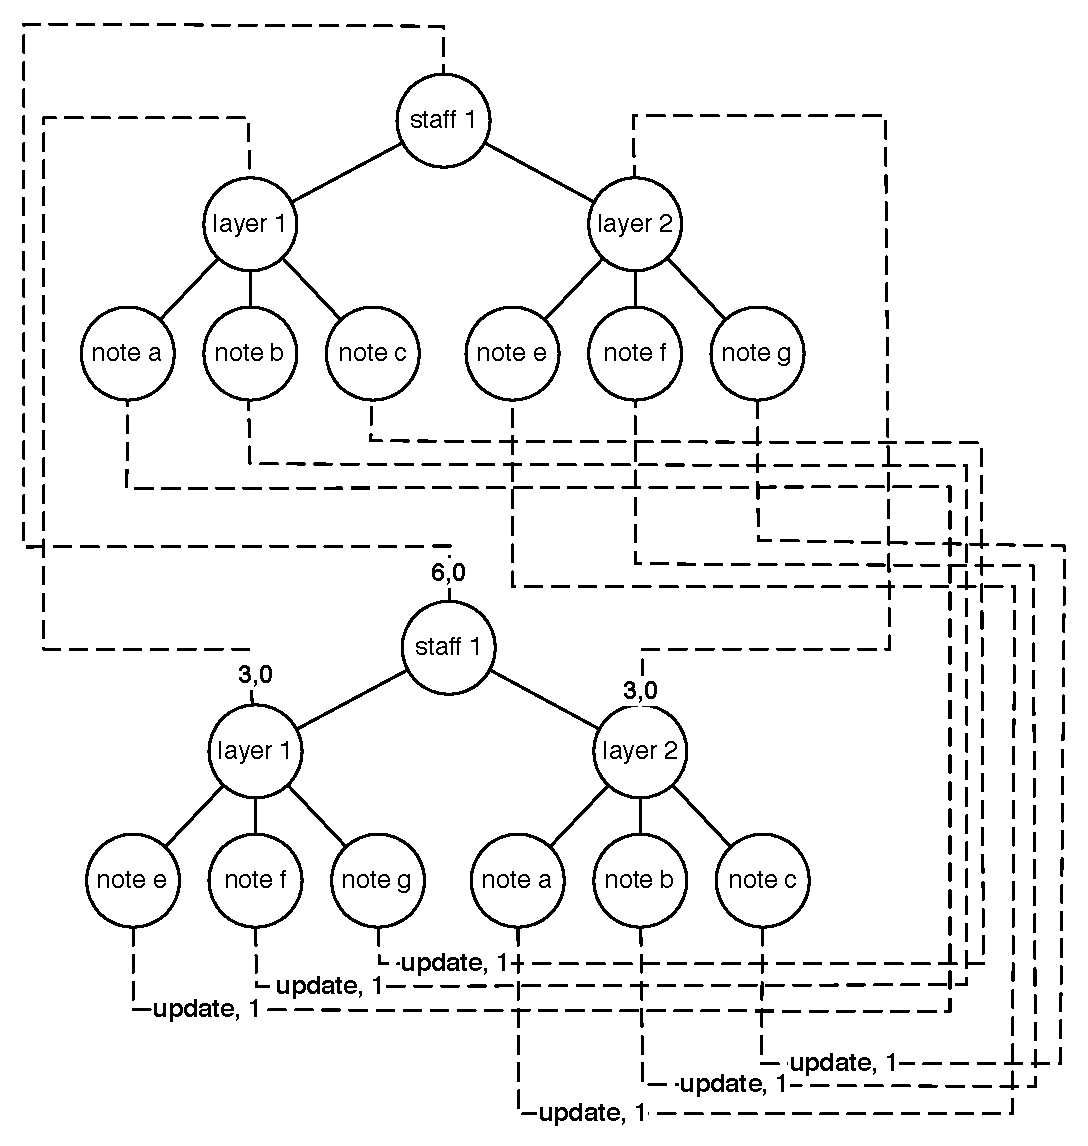
\includegraphics[width=\columnwidth]{figures/hierarchical-diff.pdf}
\caption{The figure above illustrates the output of \code{xudiff}
  applied to MEI.  A total edit distance of 6 results from updating
  the notes in layer 1 and layer 2.  Total costs are aggregated across
the hierarchical structure of the MEI text.}
\label{fig:hierarchical-diff}
\end{figure}

In contrast, Figure~\ref{fig:hierarchical-diff} illustrates an edit
script that maps one version of an MEI-encoded score to another
in terms of MEI's hierarchical object model.  As with the LCS
algorithm, the tree-based approach successfully captures the need to
switch the notes in layer 1 and layer 2.  Unlike the LCS algorithm,
however, the edit distance between individual subtrees has also been
summarized.  This can be helpful for interpretation as subtrees closer
to the root represent higher-level constructs within MEI, like voices and staves.  
As such, practitioners can interpret the comparison of the music at multiple levels 
of abstraction ranging from low-level notes (six \code{notes}, each with an edit cost of 1) 
to higher-level layers (two \code{layers}, each with an edit cost of 3) and staffs (one \code{staff}, 
with an edit cost of 6).

% Jeffrey, please see p. 121 of my thesis for citations
%  What is the related work for this approach in general and
%  specifically to music composition?


\section{Conclusions}
The recently emerged potentials of online collaborative music applications illustrate several ways a robust hierarchic diff algorithm for music can enable newly collaborative musicology, composition, and music education through document utilities \cite{wust2001architectural,Martin:2015pb,McCulloch:2015pd,Flat:aa,Baca:2015xr}.
Yet the commercial presentation of widely used digital engraving tools still conflates the act of sharing with the act of collaboration,
although these remain distinct from each other.
As a recent advertisement for the Sibelius engraving program exhorts,
``Collaborate more easily with others and distribute your compositions for the world to hear.
Share scores through email, upload and publish them as sheet music on ScoreExchange.com,
and even share your composition as a video or audio file on YouTube, Facebook, and SoundCloud'' \cite{Avid:to}.
While file exchange between music authors remains crucial for musical creativity and collaboration beyond notation,
it is time for engraving software to embrace the potentials of genuinely collaborative music document editing interfaces. But distributed collaboration on complex symbolic representations requires robust, intuitive version control algorithms and interfaces, and designers must reassess the task of music representation in light of the need for hierarchic diff. The superior performance of the Zhang and Shasha algorithm shown here suggests that purely tree-based representations, such as MEI, should be adopted for collaborative music software systems, rather than alternative representations that combine tree-based and non-tree-based models inconsistently.

%
\begin{acknowledgments}
Research conducted for the \emph{nCoda} project has been supported by Colorado College's SEGway faculty support grant.
\end{acknowledgments}

%%%%%%%%%%%%%%%%%%%%%%%%%%%%%%%%%%%%%%%%%%%%%%%%%%%%%%%%%%%%%%%%%%%%%%%%%%%%%
%bibliography here
\balance
\bibliography{tenor2017diffs}

\end{document}
